\section{RTXI Menus}

Although RTXI is dependent on Linux, it is a complete desktop application and configuration of system settings and interaction with most features are available through a graphical user interface.

The \textbf{File Menu} is used to save and load settings files that capture the entire working environment. This includes settings configured in the System Control Panel, such as channel gains, parameters set within modules, and connections between modules. Reloading a settings files will also restore the window sizes and positions at the time the file was created. Recently used settings files are also available from this menu.

\begin{figure}[h]
\begin{center}
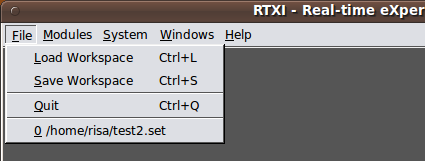
\includegraphics[width=4.5in]{fileMenu.png} 
\caption[File Menu]{The File Menu is used to save and load settings files that help you capture and recreate your working environment.} 
\end{center}
\end{figure}

The \textbf{Modules Menu} is used to load user modules or compile DYNAMO model descriptions. User modules are shared libraries that are installed to \texttt{/usr/local/lib/rtxi} during the compilation process. Choosing "Load User Module" opens a file dialog box at this location, from where users may select modules based on the *.so filename. Choosing "Load DYNAMO Model" will open a file dialog box that can be used to select a *.dynamo file containing a DYNAMO model description. This file will be parsed to generate a \cpp header and implementation file that will then be compiled to produce an RTXI module based on the \texttt{DefaultGUIModel} class. After the initial parsing and compilation, this module may then be loaded using the first menu item as with other user modules.

\begin{figure}[h]
\begin{center}
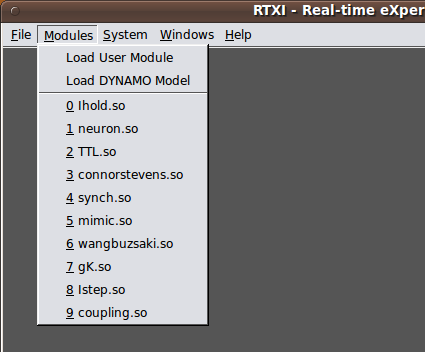
\includegraphics[width=4.5in]{modulesMenu} 
\caption[Modules Menu]{The Modules Menu is used to load user modules and compile DYNAMO models into RTXI objects.} 
\end{center}
\end{figure}

The \textbf{System Menu} is used load core RTXI system features and modules. The Control Panel is used to configure channels and set the nominal system period (or sampling rate). The Oscilloscope is the digital oscilloscope that can be used to plot any signal in real-time. The HDF Data Recorder allows users to select signals to stream to a HDF5 file in real-time. The Connector is used to specify connections between modules and the DAQ card. The Performance Measurement module displays running statistics on the computational load currently used by RTXI and how it compares to the nominal system period, or the amount of time available for performing the computations. There is also a Preferences panel for specifying commonly used directories, etc.

\begin{figure}[h]
\begin{center}
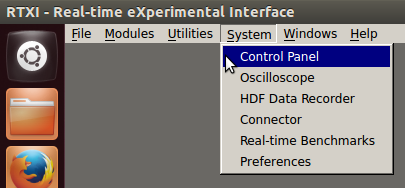
\includegraphics[width=4.5in]{systemMenu.png} 
\caption[System Menu]{The System Menu is used to access system settings and other core RTXI tools.} 
\end{center}
\end{figure}

The \textbf{Help Menu} contains important information about your system and RTXI. Choosing the "What's This" menu item turns the mouse cursor from a pointer into a question mark. In this mode, clicking on any module will display a window with contextual help, if available, about that module.

\begin{figure}[h]
\begin{center}
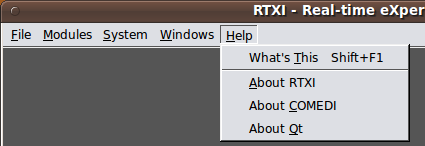
\includegraphics[width=4.5in]{helpMenu.png} 
\caption[Help Menu]{The Help Menu gives users access to contextual help for other modules and information about RTXI, COMEDI, and Qt.} 
\end{center}
\end{figure}